\documentclass[aspectratio=169]{beamer}

\usetheme{Warsaw}
\usecolortheme{default}

\usepackage[utf8]{inputenc}
\usepackage{listings}
\usepackage{xcolor}

% Configure code listings
\lstset{
    basicstyle=\ttfamily\footnotesize,
    breaklines=true,
    frame=single,
    backgroundcolor=\color{gray!10},
    keywordstyle=\color{blue},
    commentstyle=\color{green!50!black},
    stringstyle=\color{red}
}

\title{Benchmarking in bioinformatics: basics}
\author{Izaskun Mallona}
\date{\today}

\begin{document}

\frame{\titlepage}

% \begin{frame}{Overview}
%     \tableofcontents
% \end{frame}

% \section{Text and Executable Files}


\begin{frame}{Aim}
  \begin{itemize}
  \item Warm-up for exercises
  \item Seed discussion
  \end{itemize}
\end{frame}

\begin{frame}{Text files vs. executable files}
    \begin{columns}
        \column{0.5\textwidth}
        \textbf{Text Files}
        \begin{itemize}
            \item Human-readable
            \item ASCII or UTF-8 encoded
            \item Examples: \texttt{.txt}, \texttt{.csv}, \texttt{.yaml}
            \item Can be edited with text editors
            \item Platform-independent
        \end{itemize}
        
        \column{0.5\textwidth}
        \textbf{Executable Files}
        \begin{itemize}
            \item Binary format
            \item Machine-readable instructions
            \item Platform-specific (Linux amd64)
            \item Require execute permissions
            \item Examples: compiled programs
        \end{itemize}
    \end{columns}
\end{frame}

\begin{frame}[fragile]{File Permissions in Linux}
    \begin{lstlisting}[language=bash]
# View file permissions
ls -l myfile.txt
# Output: -rw-r--r-- 1 user group 1234 Nov 11 file.txt

# Make a file executable
chmod +x script.sh

# Check file type
file myfile
\end{lstlisting}
    
    \vspace{0.3cm}
    \textbf{Permission structure:} \texttt{rwx rwx rwx} (owner, group, others)
    \begin{itemize}
        \item \texttt{r} = read (4)
        \item \texttt{w} = write (2)
        \item \texttt{x} = execute (1)
    \end{itemize}
\end{frame}

\begin{frame}[fragile]{The \$PATH Environment Variable}
    \textbf{Where does Linux find executables?}
    
    The \texttt{\$PATH} variable tells Linux where to look for executable programs.
    
    \begin{lstlisting}[language=bash]
# View your current PATH
echo $PATH
# Output: /usr/local/bin:/usr/bin:/bin:/usr/sbin:/sbin

# When you type a command, Linux searches these directories
which python
# Output: /usr/bin/python
\end{lstlisting}
    
    \vspace{0.3cm}
    \textbf{Key concepts:}
    \begin{itemize}
        \item Directories are separated by colons (\texttt{:})
        \item Order matters - first match wins
        \item Software "lives" in directories listed in \texttt{\$PATH}
        \item Can be modified temporarily or permanently
    \end{itemize}
\end{frame}

\begin{frame}[fragile]{Understanding Where Software Lives}
    \begin{lstlisting}[language=bash]
# Find where a program is located
which python
# /usr/bin/python

# See all matches in PATH
which -a python
# /usr/bin/python
# /usr/local/bin/python

# Add a directory to PATH (temporary)
export PATH="/my/custom/bin:$PATH"

# Now programs in /my/custom/bin are found first
\end{lstlisting}
    
    \vspace{0.3cm}
    This is crucial for understanding Conda and Singularity environments!
\end{frame}

% \section{Git: local vs remote}

\begin{frame}{What is Git?}
    \textbf{Git} tracks changes to files
    
    \vspace{0.5cm}
    \textbf{Key concepts:}
    \begin{itemize}
        \item \textbf{Local repository}: Your copy of the project on your computer
        \item \textbf{Remote repository}: Shared copy on a server (e.g., GitHub, GitLab)
        \item \textbf{Version control}: Track all changes over time
        \item \textbf{Collaboration}: Multiple people can work on the same project
    \end{itemize}
    
    \vspace{0.3cm}
    \textbf{Why use Git?}
    \begin{itemize}
        \item Never lose work
        \item Experiment safely
        \item Collaborate effectively
    \end{itemize}
\end{frame}

\begin{frame}[fragile]{Local vs. remote repository}
    \begin{center}
        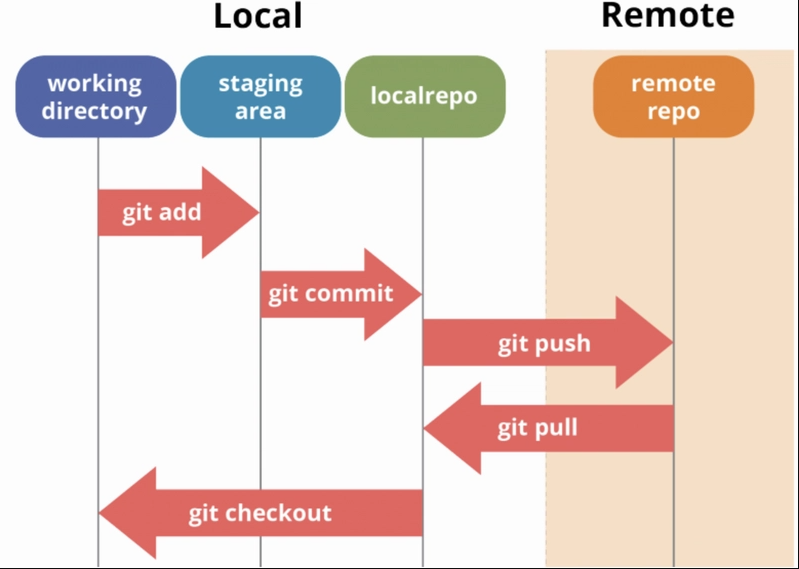
\includegraphics[width=0.6\textwidth]{git-diagram.png}
    \end{center}
    
    % \vspace{0.3cm}
    % \textbf{Workflow:}
    % \begin{enumerate}
    %     \item Edit files in \textbf{working directory}
    %     \item Stage changes with \texttt{git add}
    %     \item Save to local repo with \texttt{git commit}
    %     \item Share with remote using \texttt{git push}
    %     \item Get updates with \texttt{git pull}
    % \end{enumerate}
\end{frame}

\begin{frame}[fragile]{Git basic commands}
    \begin{lstlisting}[language=bash]
# Stage files (prepare for commit)
git add myfile.txt
git add .  # Add all changed files

# Commit (save to local repository)
git commit -m "Add analysis script"

# Push (upload to remote repository)
git push origin main

# Pull (download from remote repository)
git pull origin main
\end{lstlisting}
    
    \vspace{0.3cm}
    \textbf{Remember:} Changes stay local until you \texttt{push}!
\end{frame}

\begin{frame}[fragile]{Git workflow explained}
    \textbf{What happens locally:}
    \begin{itemize}
        \item \texttt{git add}: Stages files (marks them for commit)
        \item \texttt{git commit}: Saves snapshot to local repository
    \end{itemize}
    
    \vspace{0.3cm}
    \textbf{What happens remotely:}
    \begin{itemize}
        \item \texttt{git push}: Uploads your commits to remote server
        \item \texttt{git pull}: Downloads commits from remote server
    \end{itemize}
    
    \vspace{0.3cm}
    \begin{lstlisting}[language=bash]
# Typical workflow
git add script.py
git commit -m "Fix bug in analysis"
git push  # Now others can see your changes

git pull  # Get changes from others
\end{lstlisting}
\end{frame}

% \section{YAML files}

\begin{frame}{What is YAML?}
    \textbf{YAML} (YAML Ain't Markup Language, or Yet Another Markup Language) is a human-readable data serialization format
    
    \vspace{0.5cm}
    \textbf{Common Uses:}
    \begin{itemize}
        \item Configuration files
        \item Workflow definitions (Snakemake, Omnibenchmark)
        \item Conda environment specifications
    \end{itemize}
    
    \vspace{0.3cm}
    \textbf{Key Features:}
    \begin{itemize}
        \item Indentation-based structure (like Python)
        \item Human-friendly syntax (they claim)
        \item Supports lists, dictionaries, and nested structures
    \end{itemize}
\end{frame}

\begin{frame}[fragile]{YAML basics: Indentation Rules}
    \textbf{Critical Rule:} YAML uses \textbf{spaces for indentation}, never tabs!
    
    \begin{lstlisting}
# Key-value pairs
name: myproject
version: 1.0

# Lists (with dashes)
dependencies:
  - python
  - numpy
  - pandas

# Nested structures (2 spaces per level)
workflow:
  input:
    data: input.csv
  output:
    results: output.txt
\end{lstlisting}
    
    \vspace{0.2cm}
    \textbf{Important:} Consistent indentation (usually 2 spaces) is essential!
\end{frame}

\begin{frame}[fragile]{YAML: common patterns}
    \begin{lstlisting}
# Dictionary/mapping
config:
  threads: 4
  memory: 8GB
  
# List of dictionaries
samples:
  - name: sample1
    type: control
  - name: sample2
    type: treatment

# Multi-line strings (|)
description: |
  This is a long description
  that spans multiple lines
  and preserves line breaks

# Comments start with #
# This is a comment
key: value  # inline comment
\end{lstlisting}
\end{frame}

% \section{Snakemake}

\begin{frame}{What is Snakemake?}
    \textbf{Snakemake} is a workflow management system for reproducible and scalable data analyses
    
    \vspace{0.5cm}
    \textbf{Key Features:}
    \begin{itemize}
        \item Python-based syntax
        \item Automatic parallelization
        \item Dependency resolution
        \item Cluster and cloud execution
        \item Integration with Conda and Singularity
    \end{itemize}
    
    \vspace{0.3cm}
    \textbf{Why use workflows?}
    \begin{itemize}
        \item Reproducibility
        \item Automation
        \item Scalability
        \item Documentation
    \end{itemize}
\end{frame}

\begin{frame}[fragile]{Snakemake Basics: Rules}
    \begin{lstlisting}[language=Python]
rule process_data:
    input:
        data="data/sample.txt",
        config="config/params.yaml"
    output:
        "results/sample_processed.txt"
    shell:
        "python scripts/process.py {input.data} "
        "--config {input.config} -o {output}"
\end{lstlisting}
    
    \vspace{0.3cm}
    \textbf{Components:}
    \begin{itemize}
        \item \texttt{rule}: defines a processing step
        \item \texttt{input}: required input files
        \item \texttt{output}: files to be generated
        \item \texttt{shell}: command to execute
    \end{itemize}
\end{frame}

\begin{frame}[fragile]{Snakemake: wildcards}
    \begin{lstlisting}[language=Python]
# Process multiple samples
rule process_data:
    input:
        data="data/{sample}.txt",
        config="config/params.yaml"
    output:
        "results/{sample}_processed.txt"
    shell:
        "python scripts/process.py {input.data} "
        "--config {input.config} -o {output}"

# Target rule
rule all:
    input:
        expand("results/{sample}_processed.txt",
               sample=["sample1", "sample2", "sample3"])
\end{lstlisting}
\end{frame}

\begin{frame}[fragile]{Running Snakemake}
    \begin{lstlisting}[language=bash]
# Execute workflow
snakemake --cores 8

# Dry run (test without executing)
snakemake -n

# Create DAG visualization
snakemake --dag | dot -Tpng > dag.png

# Use specific config
snakemake --configfile config.yaml --cores 4
\end{lstlisting}
\end{frame}

% \section{Conda}

\begin{frame}{What is Conda?}
    \textbf{Conda} is a package and environment management system
    
    \vspace{0.5cm}
    \textbf{Benefits:}
    \begin{itemize}
        \item Install software without admin privileges
        \item Manage multiple versions of software
        \item Resolve dependencies automatically
        \item Create isolated environments
        \item Cross-platform (Linux, macOS, Windows) (they claim)
    \end{itemize}
    
    \vspace{0.3cm}
    \textbf{Bioconda Channel:}
    \begin{itemize}
        \item 9000+ bioinformatics packages
        \item Community-maintained
        \item Continuously tested
    \end{itemize}
\end{frame}

\begin{frame}[fragile]{Conda basics}
    \begin{lstlisting}[language=bash]
# Create a new environment
conda create -n myenv python=3.10

# Activate environment
conda activate myenv

# Install packages
conda install -c conda-forge numpy pandas matplotlib

# List installed packages
conda list

# Deactivate environment
conda deactivate
\end{lstlisting}
\end{frame}

\begin{frame}[fragile]{Conda and the \$PATH}
    \textbf{How Conda manages software locations}
    
    When you activate a Conda environment, it modifies your \texttt{\$PATH}:
    
    \begin{lstlisting}[language=bash]
# Before activation
echo $PATH
# /usr/local/bin:/usr/bin:/bin

# Activate environment
conda activate myenv

# After activation - conda's bin directory is first!
echo $PATH
# /home/user/conda/envs/myenv/bin:/usr/local/bin:/usr/bin:/bin
\end{lstlisting}
    
    \vspace{0.3cm}
    \textbf{This means:}
    \begin{itemize}
        \item Software in the active environment is found first
        \item Each environment has its own \texttt{bin/} directory
        \item Environments are \textbf{isolated} - no conflicts! (they claim)
    \end{itemize}
\end{frame}

\begin{frame}[fragile]{Conda Environment Files}
    \textbf{environment.yml} - reproducible environment specification
    
    \begin{lstlisting}
name: myanalysis
channels:
  - conda-forge
  - defaults
dependencies:
  - python=3.10
  - numpy=1.24
  - pandas=2.0
  - conda-forge::snakemake-minimal=7.32
  - matplotlib=3.7
\end{lstlisting}
    
    \begin{lstlisting}[language=bash]
# Create environment from file
conda env create -f environment.yml
\end{lstlisting}
\end{frame}

\begin{frame}[fragile]{Conda with Snakemake}
    \begin{lstlisting}[language=Python]
rule process_data:
    input:
        data="data/{sample}.txt"
    output:
        "results/{sample}_processed.txt"
    conda:
        "envs/processing.yaml"
    shell:
        "python scripts/process.py {input.data} -o {output}"
\end{lstlisting}
    
    \begin{lstlisting}[language=bash]
# Run with conda integration
snakemake --use-conda --cores 8
\end{lstlisting}
\end{frame}

% \section{Singularity}

\begin{frame}{What is Singularity? (and Apptainer)?}
    \textbf{Singularity} (Apptainer) is a container platform designed for HPC and scientific computing.
    
    \vspace{0.5cm}
    \textbf{Why Containers?}
    \begin{itemize}
        \item Complete software environment
        \item Maximum reproducibility
        \item Portable across systems
        \item No dependency conflicts
    \end{itemize}
    
    \vspace{0.3cm}
    \textbf{Singularity vs. Docker:}
    \begin{itemize}
        \item No root daemon required
        \item User permissions preserved
        \item HPC-friendly
        \item Can run Docker images
    \end{itemize}
\end{frame}

\begin{frame}[fragile]{Singularity Basics}
    \begin{lstlisting}[language=bash]
# Pull an image from Docker Hub
singularity pull docker://python:3.10-slim

# Run a command in a container
singularity exec python_3.10-slim.sif python script.py

# Run interactively
singularity shell python_3.10-slim.sif

# Build from definition file
singularity build myimage.sif myrecipe.def
\end{lstlisting}
\end{frame}

\begin{frame}[fragile]{Singularity definition files}
    \begin{lstlisting}
Bootstrap: docker
From: ubuntu:22.04

%post
    apt-get update
    apt-get install -y python3 python3-pip
    pip3 install numpy pandas matplotlib
    apt-get clean

%environment
    export PATH=/usr/local/bin:$PATH

%runscript
    echo "Running analysis pipeline"
    exec python3 "$@"

%labels
    Author yourname@yourdomain
    Version v1.0
\end{lstlisting}
\end{frame}

\begin{frame}[fragile]{Singularity and \$PATH}
    \textbf{Containers have their own \$PATH}
    
    Inside a Singularity container, software locations are isolated:
    
    \begin{lstlisting}[language=bash]
# Check PATH inside container
singularity exec myimage.sif echo $PATH
# /usr/local/bin:/usr/bin:/bin

# Container has its own filesystem
singularity exec myimage.sif which python
# /usr/bin/python (inside container)

# Outside the container, you might have different software
which python
# /home/user/conda/envs/myenv/bin/python
\end{lstlisting}
    
    \vspace{0.3cm}
    \textbf{Key point:} Container software is completely isolated from host!
\end{frame}

\begin{frame}[fragile]{Singularity with Snakemake}
    \begin{lstlisting}[language=Python]
rule process_data:
    input:
        data="data/{sample}.txt"
    output:
        "results/{sample}_processed.txt"
    singularity:
        "docker://python:3.10-slim"
    shell:
        "python scripts/process.py {input.data} -o {output}"
\end{lstlisting}
    
    \begin{lstlisting}[language=bash]
# Run with singularity
snakemake --use-singularity --cores 8
\end{lstlisting}
\end{frame}

% \section{Putting It All Together}

\begin{frame}{Reproducible Bioinformatics Workflow}
    \begin{enumerate}
        \item \textbf{Version control} (Git) for code and scripts
        \item \textbf{Workflow management} (Snakemake) for automation
        \item \textbf{Environment management} (Conda/Singularity) for dependencies
        \item \textbf{Documentation} for methods and parameters
          \item
        \item \textbf{Testing} to validate results
          \pause
        \item What about benchmarking?
    \end{enumerate}
    
    \vspace{0.5cm}
    \textbf{Best practices:}
    \begin{itemize}
        \item Use text (and open) formats when possible (easier to track)
        \item Document all software versions
        \item Share complete environments
        \item Test on different systems
    \end{itemize}
\end{frame}

% \section{Omnibenchmark}

\begin{frame}{What is Omnibenchmark?}
    \textbf{Omnibenchmark} is a platform for open and continuous benchmarking
    
    \vspace{0.5cm}
    \textbf{Key Features:}
    \begin{itemize}
        \item Modular benchmark design
        \item Automated workflow execution
        \item Continuous updates when new data/methods added
        \item Uses all the tools we've discussed!
    \end{itemize}
  \end{frame}
  
\begin{frame}{Summary}
    \begin{itemize}
        \item \textbf{Text vs. Executable Files}: Understanding file types is crucial for data analysis
        \item \textbf{YAML}: Human-readable configuration with proper indentation
        \item \textbf{Snakemake}: Automates complex workflows with dependency tracking
        \item \textbf{Conda}: Manages software and environments reproducibly
        \item \textbf{Singularity}: Provides complete containerized environments for HPC
        \item \textbf{Omnibenchmark}: Integrates all these tools for continuous benchmarking
    \end{itemize}
    
    \vspace{0.5cm}
    \textbf{Key Takeaway:} Combining these tools creates reproducible, scalable bioinformatics pipelines suitable for benchmarking and production analyses.
\end{frame}

\begin{frame}{Resources}
    \begin{itemize}
        \item Snakemake: \texttt{https://snakemake.readthedocs.io}
        \item Conda: \texttt{https://docs.conda.io}
        \item Singularity: \texttt{https://sylabs.io/docs}
        \item Omnibenchmark: \texttt{https://docs.omnibenchmark.org}
        \item YAML Tutorial: \texttt{https://yaml.org/spec/}
    \end{itemize}
\end{frame}

\end{document}
